\documentclass{article}

% Language setting
% Replace `english' with e.g. `spanish' to change the document language
\usepackage[english]{babel}

% Set page size and margins
% Replace `letterpaper' with `a4paper' for UK/EU standard size
\usepackage[scale=0.85]{geometry}


% Useful packages

\usepackage{amsmath}
\usepackage{amssymb,bm}
\usepackage{mathrsfs}
\usepackage{graphicx}
\usepackage[colorlinks=true, allcolors=blue]{hyperref}
\usepackage{graphicx} % For including images
\usepackage{caption} % For captions
\usepackage{subcaption,color} % For subfigures
\usepackage{indentfirst}
\usepackage{amsfonts}
\usepackage{parskip}
\usepackage{float,url}
\usepackage{amsthm}
\usepackage{cleveref}
\usepackage{forest}
\usetikzlibrary{automata,positioning} 
\newtheorem{theorem}{Theorem}[section]
\newtheorem{assumption}{Assumption}[section]
\newtheorem{corollary}{Corollary}[theorem]
\newtheorem{lemma}[theorem]{Lemma}
\newtheorem{proposition}[theorem]{Proposition}
\newtheorem{definition}{Definition}[section]

\definecolor{fhcolor}{rgb}{0.523, 0.235, 0.625}
\newcommand{\fh}[1]{\textcolor{fhcolor}{(SgrA: #1)}}

\title{E1 225: Introduction to Causality Models}
\author{Sahil Chaudhary}

\begin{document}
    \maketitle
    \section{Lecture 01}
    The course will deal with the notion of correlation vs causation and how do we utilize causation to develop modes.
    \textbf{Textbooks}:
    \begin{enumerate}
        \item Judia Pearl, Causality: Models, Reasoning and Inference
        \item Peter, Janzing, scholkopf, Elements of Causal Inference: Fundamentals of Learning Algorithms
    \end{enumerate}
    \subsection{Notion of Correlation:}
    Does $P(A|B)$ denote that B caused A or does it explain the probability of A given B?
    If it were to explain the causation, then consider the following:
    \begin{align*}
        P(A|B) > P(A)  &\implies \frac{P(A,B)}{P(B)}>P(A)\\
        &\implies \frac{P(A,B)}{P(A)}>P(B)\\
        &\implies P(B|A) > P(B)
    \end{align*}
    So, does this mean, A caused B and B also caused A? Definitely not, the conditional probability only explains the correlation between two events but not causality because causality is not 2 way, its 1 way implications.

    \subsection{Simpson's Paradox}
    If $\exists$ events E,C,F such that,
    \begin{align}
        P(E|C) &> P(E|C^c)\\
        P(E|C,F) &< P(E|C^c,F)\\
        P(E|C,F^c) &< P(E|C^c,F^c)
    \end{align}
    Think of it like this, people were cured given medicine worked is more than people were cured given medicine didn't work.
    But, the moment we talk about feature like gender,
    Probability that people were cured given medicine worked and they were male is less than probability of being cured given medicine didn't work and you were male. Same with female. 
    
    Then, the conclusions are absurd. How can a probability that medicine works is more on average but individually looking at the features, and summing it up, its not?

    \begin{theorem}[Sure-Thing Principle]
    An action C that increases the probability of an event E in each sub-population must also increase the probability of E in the population as whole, provided that the action doesnot change the distribution of the subpopulations.
    \begin{proof}
        Consider the population is partitioned into males and females as done before in our example.
        \begin{align}
            P(F|do(C))=P(F|do(\neg C))=P(F)
        \end{align}
        \begin{align}
            P(E|do(C),F) &< P(E|do(\neg C),F)\\
            P(E|do(C),F^c) &< P(E|do(\neg C),F^c)
        \end{align}
        Then,
        \begin{align*}
            P(E|do(C))&=P(E|do(C),F)P(F|do(C))+P(E|do( C),F^c)P(F^c|do(C))\\
            &=P(F)P(E|do(C),F)+P(F^c)P(E|do( C),F^c)P
        \end{align*}
        Similarly,
        \begin{align*}
            P(E|do(\neg C))&=P(E|do(\neg C),F)P(F|do(\neg C))+P(E|do(\neg C),F^C)P(F^c|do(\neg C))\\
            &=P(F)P(E|do(\neg C),F)+P(F^c)P(E|do(\neg C),F^C)
        \end{align*}
        Using $eq^n-5,6$,
        \begin{align*}
          P(F)P(E|do(C),F) &< P(F)P(E|do(\neg C),F)\\
            P(F^c)P(E|do(C),F^c) &< P(F^c)P(E|do(\neg C),F^c) \\ 
            \Rightarrow  P(F)P(E|do(C),F) + P(F^c)P(E|do(C),F^c) & < P(F)P(E|do(\neg C),F) +P(F^c)P(E|do(\neg C),F^c)\\
            \Rightarrow P(E|do(C)) &<P(E|do(\neg C))
        \end{align*}
    \end{proof}
    \end{theorem}

    \section{Lecture 02}
    This lecture mostly went on formalizing some basic concepts of causality for the case where the causal models contain only two variables. The lecture also breifly introduced SCMs, interventions, and counterfactuals.
    \subsection{Structural Causal Models}
    SCMs constitute an important tool to relate causal and probabilistic statements.
    \begin{definition}[Structural Causal Models]
    An SCM $C$ with graph $C \rightarrow E$ consists of two assignments:
    \begin{align}
        C &:= N_C,\\
      \label{eq:Effect}  E &:= f_{E}(C,N_E),
    \end{align}
    where, $N_E \perp N_C$.
    \end{definition}
    As you might have guessed, C is referred as cause and E as effect.

    \begin{definition}[Interventions]
        The intervened system induces another distribution, which usually differs from the observational distribution or say the two distributions become unrelated and instead of studying the system jointly, one may consider to study two systems separately.
    \end{definition}
    We may be interested in situation in which variable E is set to some value without changing the mechanism that generates C. We shall denote this by $do(E:e)$.

    The modified SCM, where \cref{eq:Effect} is replaced, entails a distribution over C that we denote by $P_{C}^{do(E:=e)}$ or $P_{C}^{\mathbf{C}:do(E:=e)}$ where the latter makes explicit that the SCM C was our starting point.\\
    \textbf{Examples:}
    Suppose that the distribution $P_{C,E}$ is entailed by an SCM $C$,
    \begin{align*}
        C&:=N_{C}\\
        E&:=5C+N_{E}
    \end{align*}
    Where, $N_{C},N_{E}\sim N(0,1)$ and graph $C \rightarrow E$. Then,
    \begin{align*}
        E_{X\sim C}[X]&= E_{X\sim N_c}[X]\\
        &=0\\
        E_{X\sim E}[X] &= E_{X \sim (5C+N_{E})}[X]\\
        &=5*0+0\\
        &=0
    \end{align*}
    AND,
    \begin{align*}
        var(C)&=var(N_{C})\\
        &=1\\
        var(E)&=var(5C+N_{E})\\
        &=E[25C^2+N_E^2+10CN_{E}]\\
        &=25+1+0\\
        &=26\\
        cov(C,E)&=E[CE]\\
        &=E[N_{C}(5N_{C}+N_E)]\\
        &=E[5N_{C}^2+N_{C}N_{E}]\\
        &=5+0\\
        &=5
    \end{align*}
    Thus, $P^C \sim N\left (\begin{bmatrix}
        0 \\
        0
    \end{bmatrix},\begin{bmatrix}
        1 && 5\\
        5 && 26
    \end{bmatrix}\right )$.\\
    Ask yourself about, $P_{C}^{C:do(E:=e)},P_{E}^{C:do(C:=c)},P_{C|E:=e}^{C},P^{C}_{E|C:=c}$
    \begin{align*}
        P_{E}^{do(C:=c)} &\sim N(E[5*c+N_{E}],E([5*c+N_{E}]-E[5*c+N_{E}])^2)\\
        &\sim N(5c,E[(5c+N_E-5c)^2])\\
        &\sim N(5c,1)
    \end{align*}
    \begin{align*}
        P_{E|C:=c} &\sim N(E[E|C=c],E[(E-E[E|C=c])^2|C=c])\\
        & \sim N(E[5*c+N_{E}],E[(E-E[5c+N_{E}])^2])\\
        & \sim N(5c,1)
    \end{align*}
    \begin{align*}
        P_C^{do(E:=e)}&\sim N(E[C],E[(C-E[C])^2]]\\
        &\sim N(0,1)
    \end{align*}
    \begin{align*}
        P_{C|E=e} &\sim N(E[C|E=e],E[(C-E[C|E=e])^2|E=e])\\
        &\sim N \left (E\left [\frac{e-N_{e}}{5} \right 
    ], E[\left( \frac{e-N_{e}}{5}-E\left [ \frac{e-N_{e}}{5}\right ]\right )^2]\right )\\
    & \sim N \left ( \frac{e}{5},E \left [ \left ( \frac{e-N_E}{5}-\frac{e}{5}\right )^2\right ]\right )\\
    & \sim N \left ( \frac{e}{5}, E \left [ \frac{N_E^2}{25}\right ]\right )\\
    & \sim N \left( \frac{e}{5},\frac{1}{25} \right)
    \end{align*}
    Thus,
    \begin{align}
        P_E^{do(C:c)}=P_{E|C=c} \quad \And \quad P_{C}^{do(E:e)} \neq P_{C|E=e}
    \end{align}
    This suggests, no matter how strongly intervene on E, the distribution of C remains what it was before.
    and the distribution of E changes if we intervene on C.
    This model behavior corresponds well to our intuition of C "Causing" E.

    We will extend the definition of SCMs in multivariate sense now. Although, to formalize the concept, we may need more lectures.
    \begin{definition}[Structural Causal Models(Multivariate)]
    A structural causal model $C:=(S,P_{N})$ consists of a collection S of $d(structural)$ assignments
    \begin{align}
      \label{eq:Structural}  X_{j}&:=f_{j}(PA_j,N_j), \quad \forall i\in [d]\\
        &\text{$N_{i}'s$ are jointly independent}
    \end{align}
    where $PA_{j} \subseteq \{ X_1,X_2,\cdots,X_{d}\} \backslash \{X_j\}$ are called parents of $X_j$; and a joint distribution $P_{N}=P_{N_1,N_2,\cdots,N_d}$ over the noise variables, which we require to be jointly independent i.e.,$P_N$ is a product distribution.
    \end{definition}
    \cref{eq:Structural} is called structural because change in one of the $f_i's$ doesn't affect the other.

    \section{Lecture 03}
    A food for thought: In traditional Machine Learning, we generally try to find or mimic the distribution and try to predict what should happen. But can we do something similar where causes and effects are involved? 

    Well, we can't. Consider SCM's $C_1$ and $C_2$, they might have same distribution but different causes. Thus, We can't.\\
    \textbf{Example}\\
    \begin{align*}
        C_1: & X=\frac{4}{10}Y+3N_x\\
        &Y=10N_y\\
        C_2: &X=5N_x\\
        &Y=\frac{8}{5}X+6N_y
    \end{align*}
    where $N_x,N_y \sim N(0,1)$.\\
    Then, the distribution of $C_1$ is,
    \begin{align*}
        P^{C_1} &\sim N\left(E\begin{bmatrix}
            X \\
            Y
        \end{bmatrix}, E \left ( \begin{bmatrix}
            X\\ Y
        \end{bmatrix}-E\begin{bmatrix}
            X \\
            Y
        \end{bmatrix}\right)^2\right)\\
        &\sim N \left ( E\begin{bmatrix}
            4N_y + 3N_x\\
            10N_y
        \end{bmatrix}, E\left[ \left ( \begin{bmatrix}
           4N_y + 3N_x\\
            10N_y 
        \end{bmatrix}-E \begin{bmatrix}
           4N_y + 3N_x\\
            10N_y
        \end{bmatrix}\right )^2\right]\right)\\
        &\sim N \left ( \begin{bmatrix}
            0\\0
        \end{bmatrix},E\left[ \begin{bmatrix}
           4N_y + 3N_x\\
            10N_y 
        \end{bmatrix}\begin{bmatrix}
           4N_y + 3N_x &&
            10N_y 
        \end{bmatrix}\right]\right )\\
        & \sim N \left ( \begin{bmatrix}
            0\\0
        \end{bmatrix},E  \begin{bmatrix}
            16N_y^2+9N_x^2+24N_xN_y  && 40N_y^2 + 30 N_x N_y \\
            40N_y^2 + 30 N_x N_y && 100N_y^2
        \end{bmatrix}\right )\\
        & \sim N \left (\begin{bmatrix}
            0 \\
            0
        \end{bmatrix}, \begin{bmatrix}
            25 && 40\\
            40 && 100
        \end{bmatrix} \right )
    \end{align*}
    and the distribution of $C_2$ is,
    \begin{align*}
        P^{C_2} &\sim N\left(E\begin{bmatrix}
            X \\
            Y
        \end{bmatrix}, E \left ( \begin{bmatrix}
            X\\ Y
        \end{bmatrix}-E\begin{bmatrix}
            X \\
            Y
        \end{bmatrix}\right)^2\right)\\
        &\sim N \left (E \begin{bmatrix}
            5N_x\\
            8N_x +6N_y
        \end{bmatrix}, E\left (  \begin{bmatrix}
            5N_x\\
            8N_x +6N_y
        \end{bmatrix}-E \begin{bmatrix}
            5N_x\\
            8N_x +6N_y
        \end{bmatrix}\right)^2 \right)\\
        &\sim N \left ( \begin{bmatrix}
            0 \\
            0
        \end{bmatrix},  E\left (  \begin{bmatrix}
            5N_x\\
            8N_x +6N_y
        \end{bmatrix}-E \begin{bmatrix}
            0\\
            0
        \end{bmatrix}\right)^2\right)\\
        &\sim N \left ( \begin{bmatrix}
            0 \\
            0
        \end{bmatrix}, E \left ( \begin{bmatrix}
            5N_x\\
            8N_x +6N_y
        \end{bmatrix} \begin{bmatrix}
            5N_x&&
            8N_x +6N_y
        \end{bmatrix} \right ) \right )\\
        &\sim N \left (\begin{bmatrix}
            0 \\
            0
        \end{bmatrix}, E \begin{bmatrix}
            25N_x^2 && 40N_x^2+30N_xN_y\\
            40N_x^2+30N_xN_y && 64N_x^2 + 36N_y^2 + 96N_xN_y
        \end{bmatrix} \right )\\
        &\sim N \left ( \begin{bmatrix}
            0 \\
            0
        \end{bmatrix}, \begin{bmatrix}
            25 && 40 \\
            40 && 100
        \end{bmatrix} \right )
    \end{align*}
    Note that $P^{C_1} \And P^{C_2}$ have the same distribution but in SCM $C_1$, $Y$ is the cause and in SCM $C_2$, $X$ is the cause. Thus, given we have found same distribution doesnot tell us anything about the causation.

    \subsection{Bayesian Network}
    \subsubsection{Preliminaries}
    Let G=(V,E) be a graph with V vertices and $E \subseteq V \times V$.
    \begin{definition}
         A graph is said to be directed graph if, 
         \begin{align*}
             PA(v)&=\{ u: (u,v) \in E\}\\
             Chi(v)&= \{u:(v,u) \in E\}
         \end{align*}
    \end{definition}
    \begin{definition}
        $v_1,v_2 \in V$ is said to be connected if $(v_1,v_2) \in E$ or $(v_2,v_1)\in E$.
    \end{definition}
    \begin{definition}
        A path is a sequence of vertices $v_1,v_2,\cdots v_k$ such that $v_i,v_{i+1}$ are connected for all $i \in [k-1]$. \\
        \noindent
        A path $(v_1,v_2,\cdots,v_k)$ is said to be \textbf{directed} if $(v_i,v_{i+1}) \in E \quad \forall i \in [k-1] $.
    \end{definition}
    \begin{definition}
        A path $(v_1,v_2,\cdots,v_k)$ is said to be \textbf{cycle} if $v_k=v_1$ and all others are distinct. 
        \\
        A cycle is called \textbf{directed} if the path is directed.
    \end{definition}
    \begin{definition}
        A graph with directed edges and no directed cycles is \textbf{directed acyclic graphs}.
    \end{definition}
    \subsubsection{Bayesian Network}
    \begin{definition}
        A bayesian network is a directed acyclic graphs whose vertices are random variables. 
    The probability distribution represented by it,
    \begin{align}
        \label{bayesian network}
        P(x_1,x_2,\cdots,x_n)&= \prod_{i=1}^{n}P(x_i|pa_i)
    \end{align}
    where $x_1,x_2,\cdots,x_n$ are random variables 
    and $pa_i$ is the set of nodes that are \textbf{Markovian Parent} of $x_i$ as described in \cref{parent def}.     
    \end{definition}

    \begin{definition}
        \label{parent def}
        Let $V=\{X_1,\cdots,X_n\}$ be an ordered set of variables, and let $P(v)$ be the joint probability distribution on these variables.
        \\ A set of variables $PA_j$ is said to be \textbf{Markovian parents} of $X_j$  if $PA_j$ is a minimal set of predecessors of $X_j$ indepedent of all its other predecessors. In other words, $PA_j$ is any subset of $\{X_1,\cdots,X_{j-1}\}$ satisfying
        \begin{align}
            \label{markov parent}
            P(x_j|pa_j)&=P(x_j|x_1,\cdots,x_{j-1})
        \end{align}
        and such that no proper subset of $PA_j$ satisfies \cref{markov parent}
    \end{definition}
    \textbf{Examples:}\\
    \begin{enumerate}
        \item 
            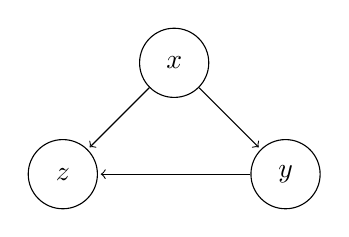
\begin{tikzpicture}[shorten >=1pt,node distance=2cm,on grid,auto] 
                \node[state](x) {$x$};
                \node[state](y) [below right= of x]{$y$};
                \node[state](z) [below left= of x]{$z$};
                \path[->]
                (x) edge node{}(y)
                (x) edge node{}(z)
                (y) edge node{}(z);
            \end{tikzpicture} 
        
        \begin{align*}
            P(x,y,z)&=P(x|pa_x)P(y|pa_y)P(z|pa_z)\\
            &=P(x)P(y|x)P(z|x,y)
        \end{align*}
        \item 
            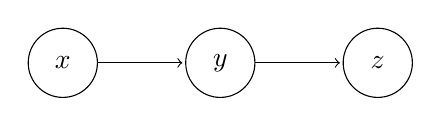
\begin{tikzpicture}[shorten >=1pt,node distance=2cm,on grid,auto] 
                \node[state](x) {$x$};
                \node[state](y) [right= of x]{$y$};
                \node[state](z) [right= of y]{$z$};
                \path[->]
                (x) edge node{}(y)
                (y) edge node{}(z);
            \end{tikzpicture} 
        
        \begin{align*}
            P(x,y,z)&=P(x|pa_x)P(y|pa_y)P(z|pa_z)\\
            &=P(x)P(y|x)P(z|y)
        \end{align*}
        \item 
         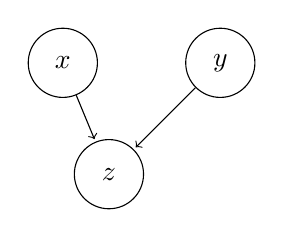
\begin{tikzpicture}[shorten >=1pt,node distance=2cm,on grid,auto] 
                \node[state](x) {$x$};
                \node[state](y) [right= of x]{$y$};
                \node[state](z) [below left= of y]{$z$};
                \path[->]
                (x) edge node{}(z)
                (y) edge node{}(z);
            \end{tikzpicture} 
        
        \begin{align*}
            P(x,y,z)&=P(x|pa_x)P(y|pa_y)P(z|pa_z)\\
            &=P(x)P(y)P(z|x,y)
        \end{align*}
        This structure is very popular and is called collider.
    \end{enumerate}
    \begin{definition}\textbf{(Markov Compatibility)}\\
        If a probability function P admits the factorization of \cref{bayesian network} relative to DAG $G$, we say that $G$ represents $P$, that $G$ and $P$ are \textbf{compatible} or that $P$ is \textbf{Markov relative} to $G$
    \end{definition}
    \subsubsection{The d-seperation criterion}
    \begin{definition}
        A path p is said to be d-separated (or-blocked) by a set of nodes Z if and only if,
        \begin{enumerate}
            \item p contains a chain $i \rightarrow m \rightarrow j$ or a fork $i \leftarrow m \rightarrow$ such that middle node $m \in Z$ or,
            \item p contains an inverted fork (or collider) $i \rightarrow m \leftarrow j$ such that the middle node $m \notin Z$ and such that no descendant of m is in Z.
        \end{enumerate}
        A set Z is said to d-separate X from Y if and only if Z blocks every path from a node in X to a node in Y.
    \end{definition}
    \textbf{Example:}
    \begin{enumerate}
        \item 
            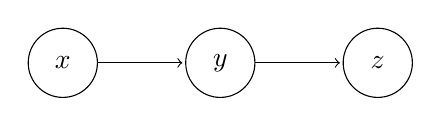
\begin{tikzpicture}[shorten >=1pt,node distance=2cm,on grid,auto] 
                \node[state](x) {$x$};
                \node[state](y) [right= of x]{$y$};
                \node[state](z) [right= of y]{$z$};
                \path[->]
                (x) edge node{}(y)
                (y) edge node{}(z);
            \end{tikzpicture} 
        
        \begin{align*}
            &x, z \text{ are d-separated by }\{y\}\\
            & \text{but } x, z \text{ are d-separated by }\{y\}\\
        \end{align*}
        \item 
         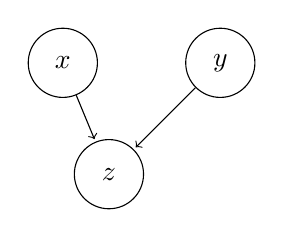
\begin{tikzpicture}[shorten >=1pt,node distance=2cm,on grid,auto] 
                \node[state](x) {$x$};
                \node[state](y) [right= of x]{$y$};
                \node[state](z) [below left= of y]{$z$};
                \path[->]
                (x) edge node{}(z)
                (y) edge node{}(z);
            \end{tikzpicture} 
      
        \begin{align*}
            &x, z \text{ are d-separated by }\{\}\\
            & \text{but } x, z \text{ are not d-separated by }\{y\}\\
        \end{align*}
    \end{enumerate}
    \textbf{Remark:} Learning in the Causal Model is equivalent to asking given data can we construct the Bayesian network of the features.
    \textbf{Lecture 04}
%	\bibliographystyle{alpha}
%	\bibliography{opt-ml}
    
\end{document}